\documentclass{article}

% Language setting
% Replace `english' with e.g. `spanish' to change the document language
\usepackage[french]{babel}
\usepackage[fleqn]{amsmath} % Aligner les équations à gauche


% Set page size and margins
% Replace `letterpaper' with`a4paper' for UK/EU standard size
\usepackage[letterpaper,top=2cm,bottom=2cm,left=3cm,right=3cm,marginparwidth=1.75cm]{geometry}

% Useful packages

\usepackage{amsmath}
\usepackage{graphicx}
\usepackage{subcaption}
\usepackage[colorlinks=true, allcolors=blue]{hyperref}

\title{TD 12 }
\author{IPESUP - PC }
\date{7 février 2024}

\begin{document}
\maketitle



\section{Ondes dans un tuyau}




\begin{figure}[h]
  \centering
  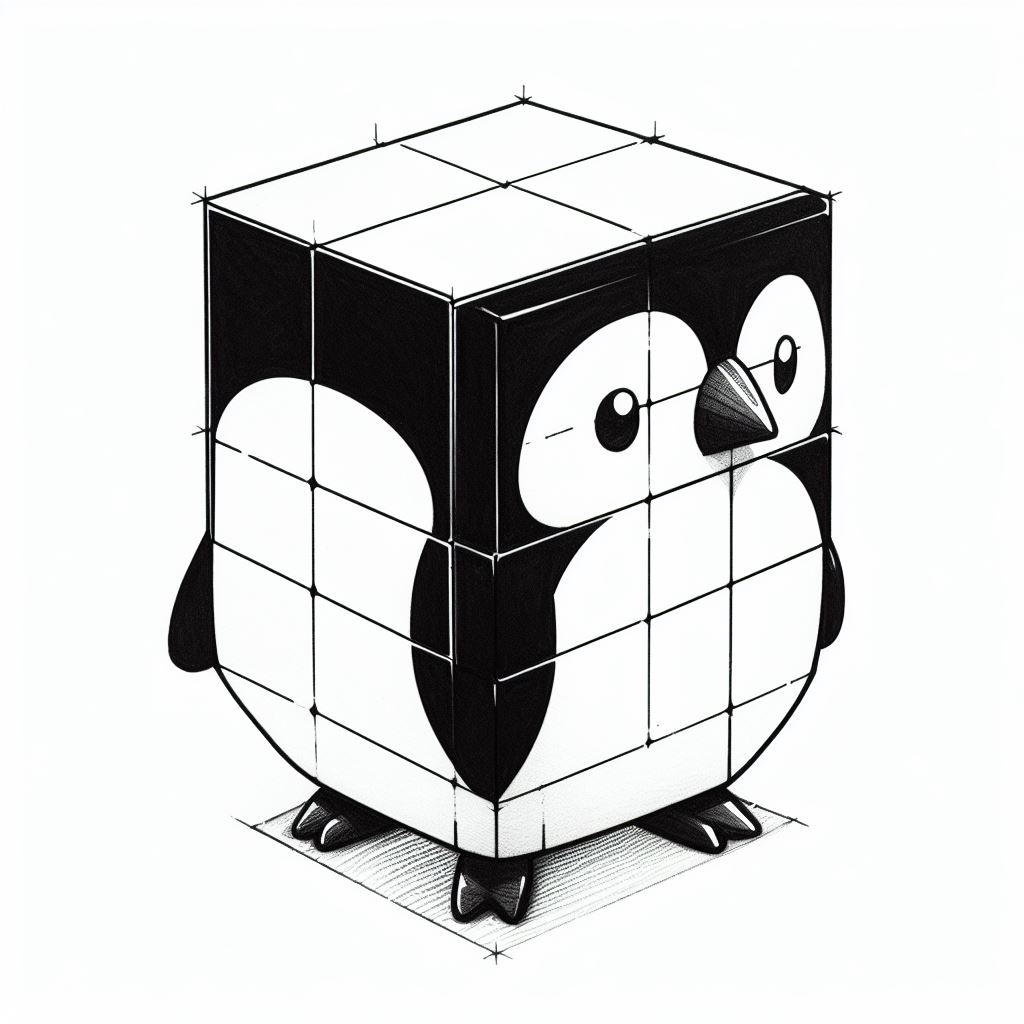
\includegraphics[width=0.4\textwidth]{pingouin_schema.jpeg}
  \label{fig:maison}
    \caption{MA FIGURE}
\end{figure}



\end{document}



\section{Exercice 1}

\section{Exercice 2}

\section{Exercice 3}

\section{ Formulaire }

\end{document}